%%%%%%%%%%%%%%%%%%%%%%%%%%%%%%%%%%%%%
%% Master Thesis - Computer Engineering
%% Copyright 2009 Ricardo Alexandre Fiorelli, Erick Poletto
%% This document is distributed by the terms of the license
%% included in the file LICENCE.
%%%%%%%%%%%%%%%%%%%%%%%%%%%%%%%%%%%%%

%%%%%%%%%%%%%%%%%%%%%%%%%%%%%%%%%%%%%
%% Third Chapter
%% Methodology
%%%%%%%%%%%%%%%%%%%%%%%%%%%%%%%%%%%%%

\chapter{Methodology} \label{chap3:methodology}

\section{Overview} \label{sec3:overview}
    This research was conducted in order to determine how much energy a computer's component, such as CPU, Memory, Hard Drives, spends and, also, how much it would have an effect in the cost of the Data Center. The advantages and disadvantages as well as the reliability of these measures played also an important role in the objectives of this thesis work.

\subsection{Research Design} \label{sec3:research_design}

\subsection{Participants} \label{sec3:participants}

\section{Energy Management Tools} \label{sec3:energy_management_tools}
\subsection{SiSoftware SANDRA} \label{sec3:sandra}
    SANDRA was the main software utilized to benchmark the data in this thesis work. It contains a huge database of components to make sure the benchmarks provided have the best results and accurate comparisons.
    
    SiSoftware Sandra\footnote{The \textbf{S}ystem \textbf{AN}alyser, \textbf{D}iagnostic and \textbf{R}eporting \textbf{A}ssistant} is an information \& diagnostic utility. It provides most of the information (including undocumented) one need to know about their hardware, software and other devices whether hardware or software.
    
    The software goes beyond the point of other Windows Utilities, by giving the user, the possibility of benchmarking and comparing at both high and low level the computer devices. Moreover, it is a tool for monitoring the performance on systems and even benchmarking many parts of the computer, this includes, CPU\footnote{Central Processing Unit}, memory, hard disks, CD/DVD ROM, network, PSU\footnote{Power Supply Unit}, etc. For that reason, it is considered one of the most complete benchmarking tools available.
    
    Besides the benchmarking, Sandra also provides access to information about the Hardware, including the Motherboard, processor, disks, printers, etc; and Software, such as, key softwares (web browsers, e-mail program, etc.), OS information, processes, memory usage and more.
    
    The detailed list of modules utilized by SiSoftware Sandra can be found in Appendix~\ref{app:sandra_modules}.
    
    Furthermore, the Sandra has a great functionality that is a catalog of pricing, which, in addition to the power consumption and other important characteristics, the best combination (which means the most green) of devices can be chosen to the server.
    
\subsection{Other Tools} \label{sec3:other_tools}
    In order to make sure the best option was chosen it was used another tools, other than Sandra, with the intention of complementing the features and results of the benchmarks provided. 
    
\subsubsection{Energy Measurement Instrument} \label{sec3:measurement_instrument}

    \begin{figure}[!h]
        \centering
            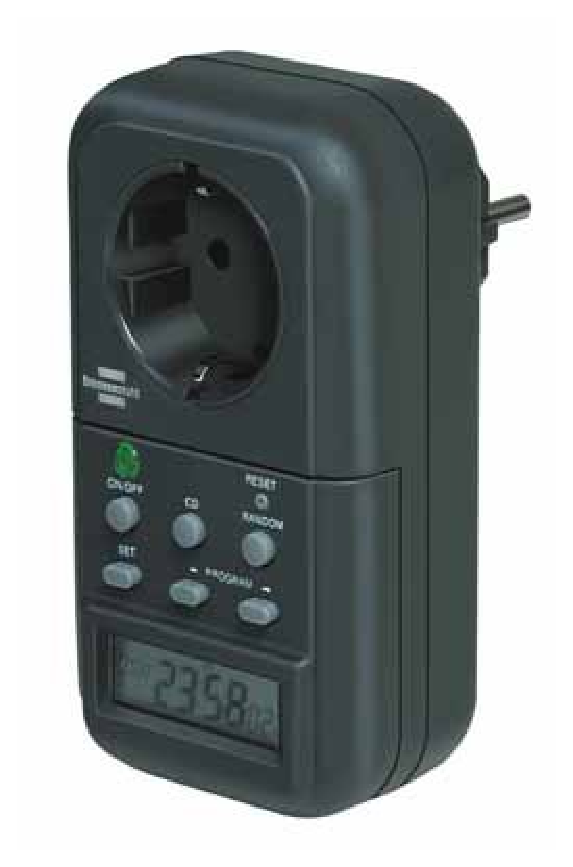
\includegraphics[scale=0.6]{graphics/energy_measurement_instrument}
            \caption{Energy Measurement Instrument}
            \label{fig:energy_measurement_instrument}
    \end{figure}
This is the instrument used for comparing with the results of the benchmarks given by Sandra. 

\subsubsection{WebSPHINX - A Personal, Customized Web Crawler} \label{sec3:websphinx}
    WebSPHINX\footnote{Website-Specific Processors for HTML Information Extraction} is a Java class library used for web crawling. It provides a way to browse and process web pages automatically.
    
    This piece of software was used to establish the pricing, linking it with the MPN\footnote{Manufacturer's Part Number}, and, afterwards, composing the database explained in \ref{sec4:analysis}. 

\subsubsection{CPU-Z} \label{sec3:cpu-z}
    CPU-Z detects information about the CPU, RAM Memory, motherboard, chipset and more. That program was used to complete the database with missing information about the components.

\subsubsection{PlateSpin - Recon} \label{sec3:power_recon}
    This software did not compose the ones used for doing this thesis. Yet, it is important to notice this, because it is almost the same of Sandra, but it provides a more incisive work on Data Centers in general. It provides workload profiling, analysis and planning of complex server consolidation, disaster recovery, capacity planning, asset management and green data center initiatives. It also provides forecasting for optimizing the data center by collecting hardware, software and services inventory for all server workloads. Furthermore, it results an statistics work for the server workloads running on data center and how their resources are being used.
    
    For the reason that it was needed to compare the components, in order to draw a picture of the most suitable components to be used. It was chosen Sandra, which has a great database of components.

\section{Measurement Methodology} \label{sec3:measurement_methodology}

